\section{Description générale de la nouvelle application}
\label{sec:Description generale de l'application}
L'application Espace Recruteur permet à des recruteurs d'entreprise de publier dans la partie publique du site Cadremploi une offre destinée à des cadres et cadres supérieurs.
Néanmoins, il s'agit de plus qu'un simple formulaire.
En effet, en plus du remplissage d'un formulaire esthétique permettant de rédiger l'offre qu'il souhaite déposer, l'espace recruteur propose plusieurs services.
Le recruteur ayant un compte sur l'espace recruteur du site Cadremploi dispose d'un panneau de contrôle lui permettant de gérer ses offres et d'en consulter les informations associées.
De plus, une équipe de Figaro CLASSIFIEDS supervise via une seconde application dédiée, la publication des offres.

%---------------------------------------------------------------
\subsection{Backoffice}
\label{sub:Backoffice}
Le backoffice est une application interne à Cadremploi permettant de gérer toutes les offres existantes.
Chaque offre créée par un recruteur se doit d'être complètement sous contrôle de manière à pouvoir gérer tout cas inattendu.
Ainsi, cette application est développée en parallèle à l'espace recruteur par notre équipe, comme un panneau de gestion de toutes offres rédigées par les recruteurs.
Un backoffice existe déjà pour l'espace recruteur courant, mais il est aussi agé que l'espace recruteur actuel et les nouveautés apportées dans cette nouvelle version demandent une telle adaptation que le développement d'un nouveau backoffice est nécessaire.
\begin{figure}[b]
  \begin{center}
    \hspace*{-1in}
    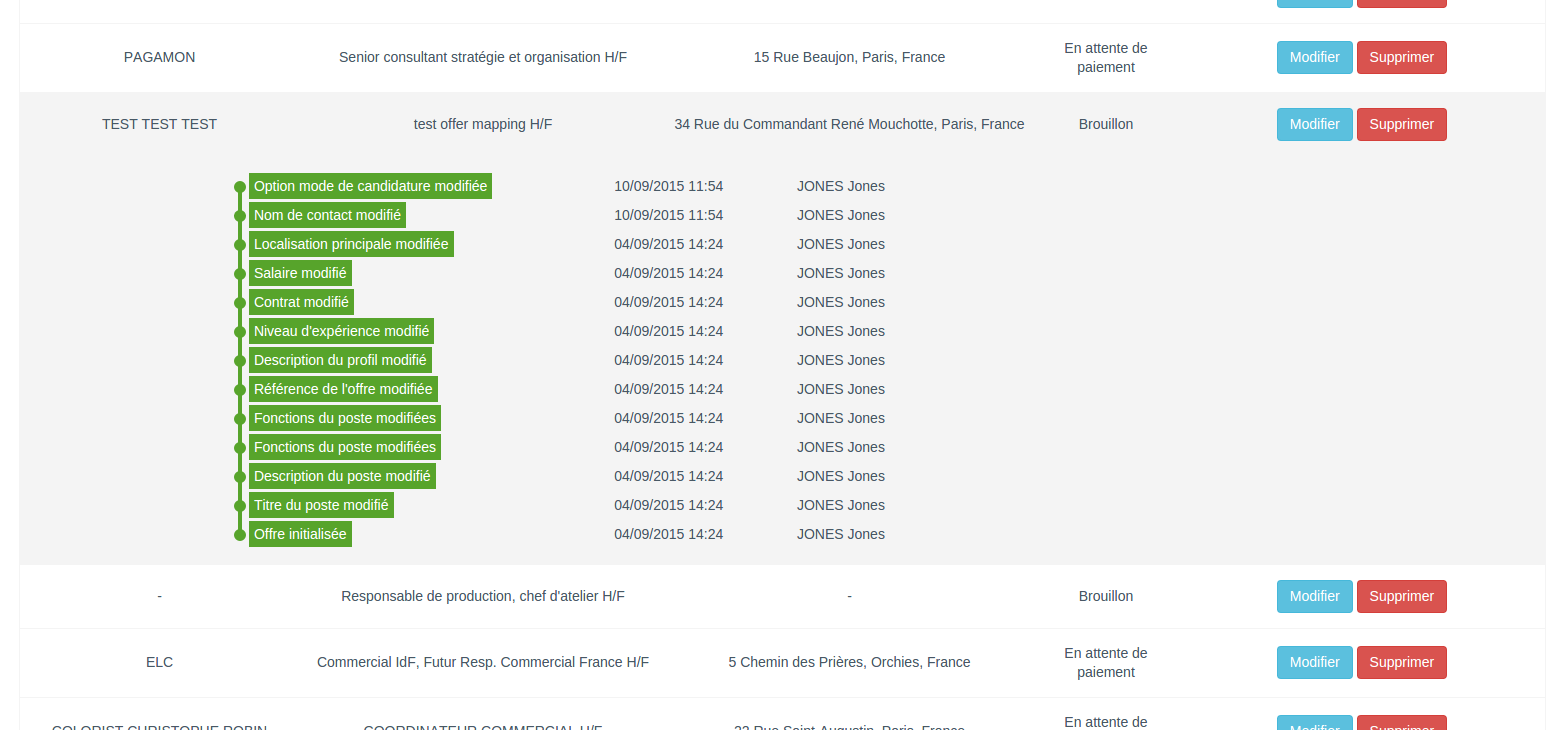
\includegraphics[width=1.3\textwidth]{Pictures/backoffice.png}
    \label{pic:suivi client backoffice}
    \caption{Le suivi de l'évolution du client dans le backoffice}
  \end{center}
\end{figure}
Les fonctionnalités nécessaires sur ce nouveau backoffice sont:
\begin{itemize}
  \item Le login "en tant que" un autre recruteur:
  Il est possible depuis le backoffice de se connecter pour éditer une offre comme si on était le recruteur qui l'avait rédigé et ainsi y apporter tous les changements désirés.
  Cela permet un contrôle parfait sur une offre puisque toutes les actions permises pour le recruteur le sont aussi pour le superviseur.
  Il est ainsi possible de gérer les problèmes potentiels en effectuant les modifications nécessaires à la place du recruteur.
  \item La gestion de la discrimination des offres en fonction de leur contenu:
  Une des fonctionnalité de l'espace recruteur est la détection de termes discriminants dans les champs textuels d'une offre.
  Ainsi, si une offre est détectée comme présentant des termes discriminants, elle n'est pas directement publiée sur le site.
  Une offre discriminante ne sera visible que sur le backoffice d'où elle sera relue par des responsables de la relation client (RC).
  Les RC sont chargés de traiter, si nécessaire avec le client, les offres discriminantes afin de les rendre acceptables dans les plus brefs délais.
  Le but de cette procédure est de ne pas handicaper le client et de régler les problèmes rencontrés rapidement.
  \item Le suivi de l'évolution du client au cours de la création de son offre (\ref{pic:suivi client backoffice}).
  Cette fonctionnalité permet à un RC de pouvoir se rendre compte du parcours du client lorsque celui-ci rédige son offre (l'ordre dans lequel il a rempli les champs, le temps qu'il a mis à les remplir, ...) et donc de pouvoir l'aider au mieux lors de sa prise de contact.
  Les événements de modification effectués par le recruteur au cours de sa saisie sont donc visibles par le RC consultant une offre donnée.
\end{itemize}

%---------------------------------------------------------------
\subsection{Le panneau de contrôle du recruteur}
%---------------------------------------------------------------
\subsubsection{Statistiques}
\label{subs:Statistiques}
\begin{figure}[h]
  \begin{center}
    \hspace*{-1in}
    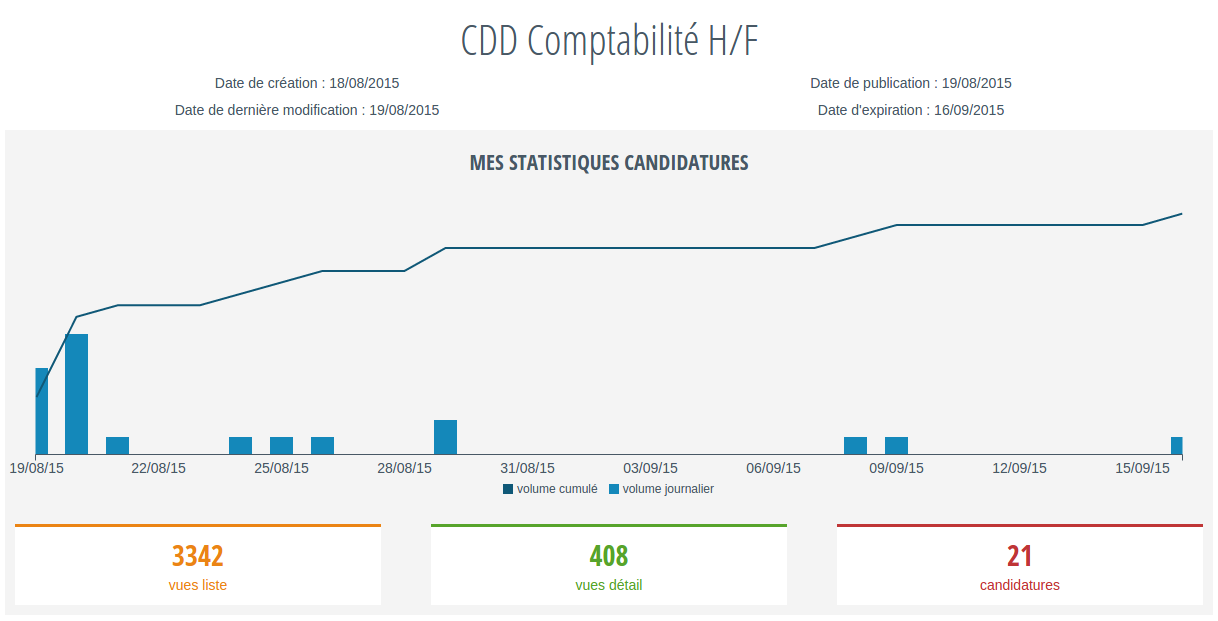
\includegraphics[width=1.2\textwidth]{Pictures/stats.png}
    \label{pic:suivi client backoffice}
    \caption{Les mesures statistiques proposées sur l'espace recruteur}
  \end{center}
\end{figure}
Un système de statistiques mesurant la rentabilité de l'annonce est mis en place pour que le recruteur puisse suivre l'évolution de son offre.
Ce système de statistiques est totalement externalisé de l'application et a été développé par une équipe différente de celle de Cadremploi.
Il permet ainsi à tout FIGARO CLASSIFIEDS de récupérer des statistiques sur l'utilisation de l'espace recruteur de Cadremploi.
L'incorporation de cette API de statistiques ainsi que la récupération des informations nécessaires étaient deux points importants dans le développement du nouvel Espace Recruteur.
%---------------------------------------------------------------
\subsubsection{Label qualité}
\label{subs:Label qualité}
Une des autres manière de garantir la qualité des offres présentes sur Cadremploi est la création d'un label qualité.
Il s'agit en somme d'un système de classement des offres qui fera passer les offres considérées comme étant de qualité devant celles ne l'étant pas dans la liste visible sur l'espace public.
Cela permet d'inciter le recruteur à proposer des annonces avec des descriptions complètes ou des vidéos présentant l'entreprise, de manière à proposer un taux d'offres attractives plus important.
Cette fonctionnalité n'est pas implémentée à ce jour.
%---------------------------------------------------------------
\subsubsection{Event sourcing}
\label{subs:Event sourcing}
Enfin, une gestion fine des modifications apportées par les recruteurs à leurs offres sera faite.
En effet, chaque modification faite par un recruteur sur son annonce sera enregistrée de manière à suivre son évolution au cours du processus de mise en ligne d'annonce.
Elle permettra par exemple aux RC traitant avec les recruteurs de pouvoir comprendre clairement la façon dont ils ont procédés et ainsi mieux les aider.
Cette gestion permet de plus, comme je l'expliquerai plus tard, de pouvoir revenir à un état précédent d'une offre, dans le cas d'un recruteur ayant fait une erreur de manipulation.

\paragraph{}
Seule la mise en place du pattern Event Sourcing avait débuté à mon arrivée et j'ai ainsi participé au développement des autres fonctionnalités.
